\section{Righe Spettrali}\label{sec:righe-spettrali}

\subsection{Opacità per l'atmosfera stellare}\label{sec:opacità-atmosfera}
Un parametro importante per la determinazione di un modello per l'atmosfera stellare è l'opacità, già discussa nel par.~\ref{sec:opacità}. Ripassiamo i concetti principali. I processi che determinano l'opacità di una struttura sono:
\begin{description}
    \item[BB] discusso nel par.~\ref{sec:bound-bound}. Avviene a una determinata lunghezza d'onda, secondo l'eq.~\eqref{eq:lunghezza-BB}. È responsabile delle \emph{righe di assorbimento}, poiché determinano la mancanza di flusso a una determinata lunghezza d'onda.
    \item[BF] discusso nel par.~\ref{sec:bound-free}. Contribuisce all'opacità del \emph{continuo}.
    \item[FF] discusso nel par.~\ref{sec:free-free}. Contribuisce all'opacità del \emph{continuo}.
    \item[E] discusso nel par.~\ref{sec:electron-scattering}. Contribuisce all'opacità del \emph{continuo}.
\end{description}
In particolare, nelle atmosfere le temperature sono sufficientemente basse affinché i fotoni possano essere poco energetici e possano eccitare gli elettroni degli atomi, lasciandoli in stati legati. Dunque il fenomeno del BB, che negli interni stellari trascuravamo a causa delle elevate temperatura, sarà determinante nelle atmosfere. La velocità di variazione dell'opacità con la lunghezza d'onda determina come l'opacità stessa si manifesta, ovvero in forma di righe di assorbimento o nel continuo. Vediamo degli esempi.

\paragraph{Esempio--Serie di Balmer}
\paragraph{Esempio--Balmer Jump}

\subsection{Continuo spettrale e righe spettrali di assorbimento}

\subsection{Classificazione spettrale delle stelle}
Come visto nel par.~\ref{sec:opacità-atmosfera}, l'\emph{atmosfera} stellare è dove si formano il \emph{continuo spettrale} e le \emph{righe spettrali di assorbimento}. Le righe di assorbimento, in particolare, sono degli osservabili fondamentali perché è dalla loro intensità che possiamo misurare l'\emph{abbondanza} dei diversi elementi chimici. Si faccia attenzione al seguente fatto: la presenza o meno di una data riga spettrale \emph{non} dipende dalla presenza o meno di quel dato elemento, ma è fortemente modulata dalla \emph{temperatura}. Vediamo di chiarire il fatto.

Ovviamente, se un elemento non è presente nella struttura stellare, lo spettro non potrà mostrare le sue righe. Tuttavia, l'assenza di righe di un dato elemento \emph{non necessariamente} significa che quel dato elemento è assente: potrebbe esserci, ma la \emph{temperatura} non è tale da far manifestare le sue righe. Infatti, le righe di assorbimento sono dovute a fenomeni di eccitazioni o ionizzazioni della materia e, come noto,  il numero di stati eccitati o ionizzati dipende primariamente dalla temperatura. Se, ad esempio, la temperatura non è sufficientemente alta da far sì che tutti gli atomi di un dato elemento siano ionizzati, non potrò mai vedere la riga di assorbimento di tale elemento, anche se esso è presente.

In definitiva, è la temperatura che modula il manifestarsi delle righe spettrali, ovvero è la \emph{temperatura} che determina il \emph{tipo spettrale} delle stelle. Dunque, le stelle sono classificate in base al loro tipo spettrale, ovvero in base alla presenza e all'intensità delle varie righe spettrali, il quale, a sua volta, riflette il valore della temperatura atmosferica della stella.

\begin{figure}
    \centering
    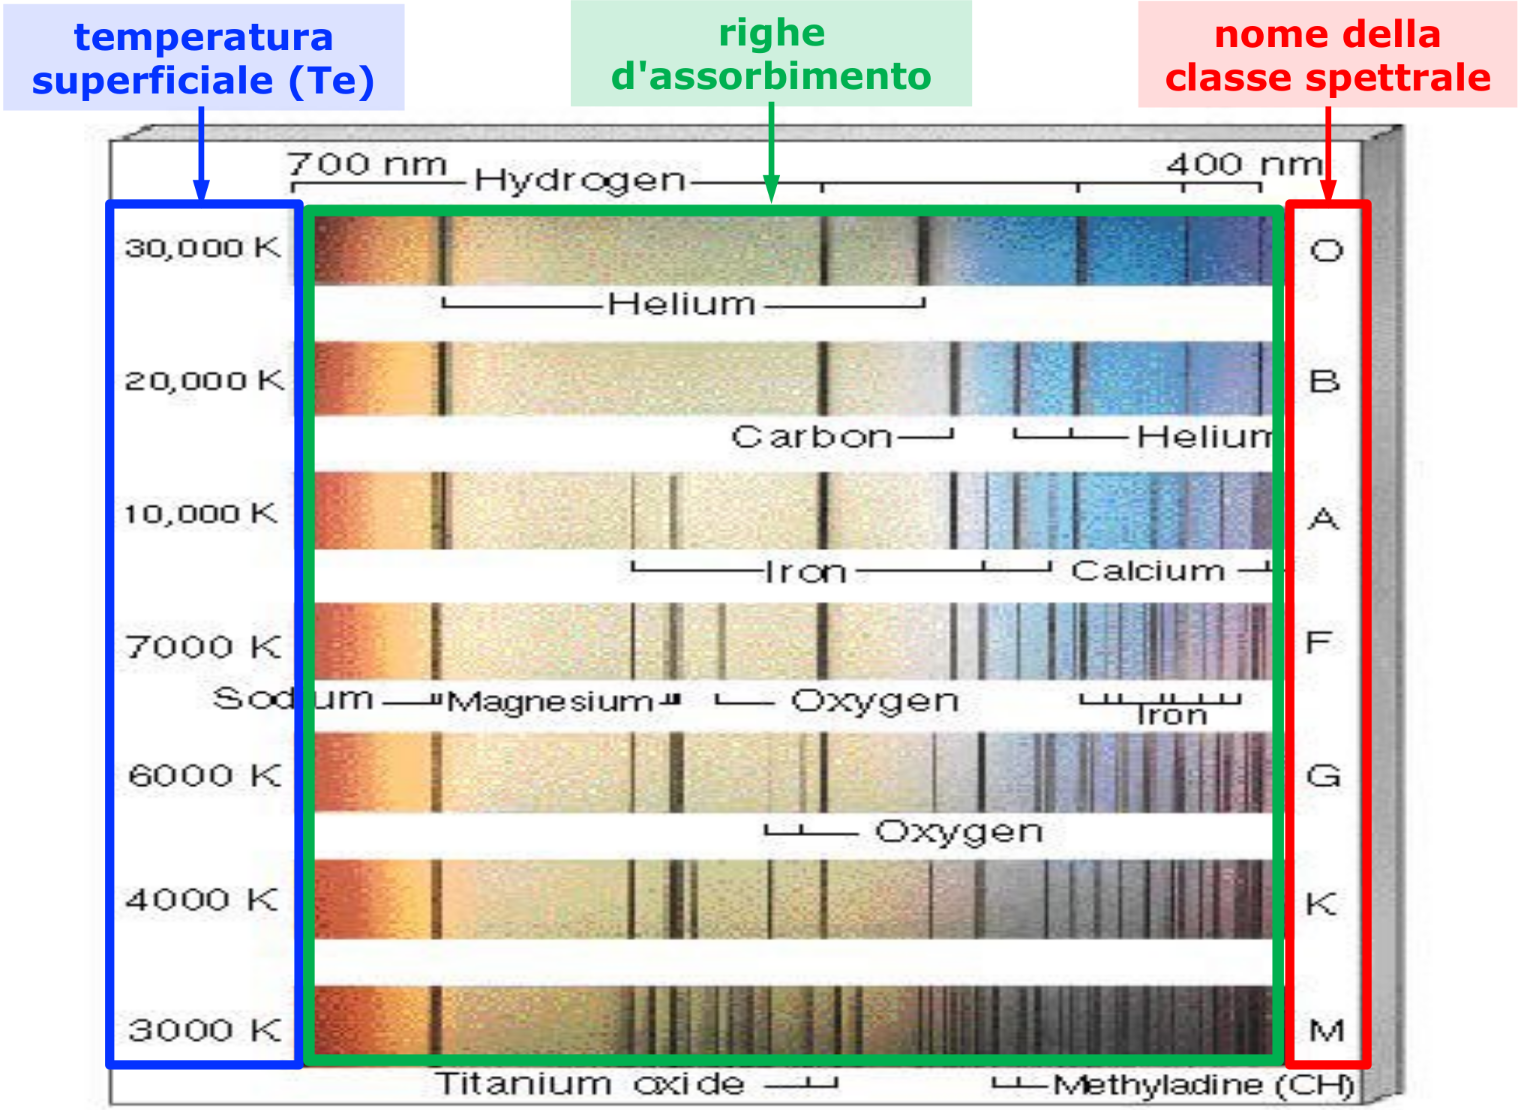
\includegraphics[width=0.7\textwidth]{immagini/classificazione-spettrale-stelle.png}
    \caption{Classi spettrali principali.}
    \label{fig:classificazione-spettrale-stelle}
\end{figure}

\begin{figure}
    \centering
    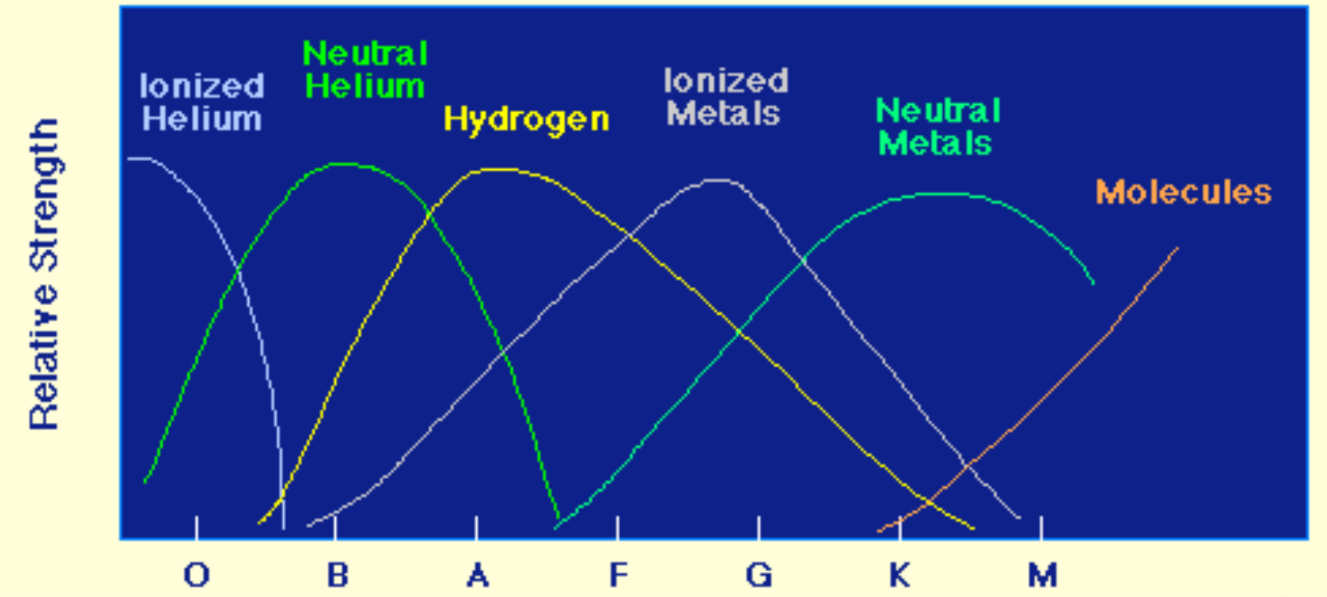
\includegraphics[width=0.7\textwidth]{immagini/classificazione-spettrale-stelle-2.png}
    \caption{Classi spettrali principali.}
    \label{fig:classificazione-spettrale-stelle-2}
    
\end{figure}

Nelle fig.~\ref{fig:classificazione-spettrale-stelle} e fig.~\ref{fig:classificazione-spettrale-stelle-2} sono rappresentate le principali \emph{classi spettrali}, elencate anche di seguito:
\begin{description}
    \item[O] $T_e > \SI{25000}{K}$
    \item[B] $ \SI{11000}{K} < T_e < \SI{25000}{K}$: ???
    \item[A] $ \SI{7500}{K} < T_e < \SI{11000}{K} $: ???
    \item[F] $ \SI{6000}{K} < T_e < \SI{7500}{K} $: ???
    \item[G] $ \SI{5000}{K} < T_e < \SI{6000}{K} $: ???
    \item[K] $ \SI{3500}{K} < T_e < \SI{3000}{K} $: ???
    \item[M] $ \SI{3500}{K} < T_e < \SI{3000}{K} $: ???
\end{description}
Si può ricordare tale lista con la seguente frase: \emph{"O,B,A, Fine Girl Kiss Me"}.

Come detto precedentemente, una data riga di assorbimento è presente o assente nello spettro a seconda del numero di atomi nei diversi stati eccitati o ionizzati di quel dato elemento. Tale numero dipende in primo luogo dalla temperatura e viene stimato attraverso:
\begin{description}
    \item[Equazione di Boltzmann]: percentuale di atomi in un dato stato di eccitazione. Risponde alla domanda: "quale frazione di atomi con elettroni legati si trova in un dato stato eccitato?"
    \item[Equazione di Saha]: percentuale di atomi in un dato stato di ionizzazione. Risponde alla domanda: "questo elemento ha ancora elettroni legati?"
\end{description}

\subsection{Equazione di Boltzmann}
Come suggerito nel precedente paragrafo, l'\emph{equazione di Boltzmann} fornisce la percenutale di atomi in un dato stato di eccitazione. In particolare, per ogni specie chimica, considera gli atomi ionizzati $j$--volte ($N_j$) e fornisce la frazioen di quelli che sono eccitati $i$--volte ($N_{ji}$):
\begin{equation}\label{eq:equazione-boltzmann}
    \dfrac{N_{ji}}{N_j} = \dfrac{g_i}{{U_j}(T)} 10^{-\theta \chi_i} 
\end{equation}
dove:
\begin{description}
    \item[$N_j$]: numero di atomi nello stato di ionizzazioni j (ovvero ionizzati $j$--volte).
    \item[$N_{ji}$]: numero di atomi nello stato di ionizzazione j, che si trovano nello stato di eccitazioni i (ovvero ionizzati $j$--volte \emph{ed} eccitati $i$--volte).
    \item[$g_i$]: peso statistico del livello energetico i.
    \item[$\theta \equiv \frac{5040}{T} \si{eV^{-1}}$], con $T$ espressa in $\si{K}$.
    \item[${U_j}(T)$]: funzione di partizione per lo stato di ionizzazione j.
    \item[$\chi_i$]: potenziale di eccitazione dal primo livello energetico disponibile al livello energetico $i$.      
\end{description}
Notiamo che l'espressione è dipendente dalla struttura dell'atomo, attraverso i termini $g_i$, ${U_j}(T)$ e $\chi_i$, e dalla temperatura. In definitiva, la percentuale è tanto maggiore quanto più alta è $T$ e quanto più basso è il potenziale di eccitazione $\chi_i$. Vediamo, ora, i vari termini con maggior dettaglio.

\paragraph{Peso statistico}
Il peso statistico $g_i$ del livello energetico $i$--esimo rappresenta il numero di livelli energetici degeneri, ovvero alla stessa energia. Per gli atomi idrogenoidi si ha:
\begin{equation*}
g_i = 2 i^2
\end{equation*}
e si ottengono i noti risultati per cui il nel livello fondamentale ($i=1$) si ha $g_1 = 2$, ovvero possono alloggiare $2$ elettroni di spin opposto, mentre nel primo livello eccitato, $i=2$, vale $g_2=8$ e possono alloggiare $2$ elettroni nell'orbitale s e $6$ elettroni nell'orbitale p, e così via.

\paragraph{Funzione di partizione}
La funzione di partizione per lo stato di ionizzazione $j$--esimo, ${U_j}(T)$, è una sommatoria dei pesi statistici ($g_i$) di tutti i livelli energetici pesati con un termine che dipende dalla temperatura, ovvero:
\begin{equation*}
    {U_j}(T) = \sum_i g_i 10^{-\theta \chi_i}
\end{equation*}

\paragraph{Potenziale di eccitazione}
nell'equazione~\eqref{eq:equazione-boltzmann}, $\chi_i$ rappresenta il potenziale di eccitazione dal primo livello energetico \emph{disponibile} al livello energetico $i$--esimo. Vediamo cosa si intende per primo livello disponibile, il quale dipenderà dal livello di ionizzazione, j. Consideriamo, ad esempio, \ce{NeI}, ovvero il neon neutro. Esso ha 10\ce{e^-} legati, in cui $2$\ce{e^-} si trovano nel livello $n=2$ e $8$\ce{e^-} si trovano nel livello $n=2$. Essendo, dunque, i primi due livelli totalmente occupati, il primo livello disponibile sarà $n=3$. Nel caso di \ce{NeII}, ovvero del neon ionizzato $1$ volta, il primo livello disponibile è $n=2$, non essendo questa volta occupato del tutto. 

Per gli atomi idrogenoidi, il potenziale di eccitazione tra due livelli energetici $a$ e $b$, con $a<b$, è:
\[
    \chi_{ab} = Z^2 \bigl( \dfrac{1}{{n_a}^2} - \dfrac{1}{{n_b}^2} \bigr) \times \SI{13.6}{eV}
\]
con $Z$ il numero atomico. Essendo il primo livello energetico disponibile il livello fondamentale, rappresentato da $a=1$, si ha:
\[
  \chi_i = Z^2 \bigl( 1-\dfrac{1}{i^2}  \bigr)  \times \SI{13.6}{eV}
\]

\subsection{Equazione di Saha}
Per ogni specie chimica, l'\emph{equazione di Saha} fornisce la percentuale di atomi ionizzati $j+1$--volte ($N_{j+1}$) rispetto al numero di atomi ionizzati $j$--volte ($N_j$):
\begin{equation}\label{eq:equazione-saha}
    \log \dfrac{N_{j+1}}{N_j} = -0.176 - \log P_e - \theta \chi_i + 2.5 \log T + \log \dfrac{{U_{j+1}}(T)}{{U_j}(T)}
\end{equation}
dove:
\begin{description}
    \item[$N_j$, $N_{j+1}$]: numero di atomi nello stato di ionizzazione $j$ e $j+1$, ovvero contigui.
    \item[$P_e$]: pressione elettronica, ovvero esercitata dalla componente elettronica del gas.
    \item[$\theta \equiv \frac{5040}{T} \si{eV^{-1}}$], con $T$ espressa in $\si{K}$.
    \item[$\chi_i$]: potenziale di ionizzazione dell'atomo ionizzato $j$--volte. ERRORE FORSE, NON DOVREBBE ESSERE CHI J??????
    \item[${U_j}(T)$, ${U_{j+1}}(T)$]: funzioni di partizione per gli stati di ionizzazione $j$ e $j+1$.
\end{description}
Si faccia molta attenzione a cosa si riferisce l'eq.~\eqref{eq:equazione-saha}. Essa \emph{non} permette di calcolare il numero di atomi in un certo stato di ionizzazione ( $N_j$ ) rispetto al numero totale ($N$) di atomi di quella specie, che sarebbe equivalente a $N_j / N$, tuttavia essa calcola il rapporto tra il numero di atomi in due stati di ionizzaione contigui ($j+1$ e $j$), equivalente a $N_{j+1} / N_j$. Per ottenere $N_j / N$ sono necessarie applicazioni successive dell'equazione di Saha tra due stati di ionizzazione contigui.

\subsection{Frazione di atomi attivi}
In pratica, mettendo insieme le due equazioni, per ogni equazione chimica:
\begin{itemize}
    \item l'equazione di Saha~\eqref{eq:equazione-saha} mi dice se, a quella data temperatura $T$ esistono atomi che non sono completamente ionizzati, cioè che hanno ancora elettroni legati
    \item se ciò è vero, l'equazione di Boltzmann~\eqref{eq:equazione-boltzmann} mi dice se, a quella data temperatura $T$ gli elettorni legati sono nello stato fondamentale o in quale livello di eccitazione
\end{itemize}
Insieme, le eq.~\eqref{eq:equazione-saha} e~\eqref{eq:equazione-boltzmann} forniscono la \emph{frazione di atomi attivi} $N_a$ (che generano le righe spettrali) rispetto al totale di atomi di quella specie. È possibile misurare $N_a$ attraverso un'analisi spettroscopica delle righe spettrali, dunque, in definitiva, usando le equazioni di Saha e Boltzmann è possibile ricavare l'\emph{abbondanza} di quel dato elemento chimico. 

\subsection{Velocità radiale}
\subsection{Abbondanze chimiche}
\subsubsection{Larghezza equivalente}
\subsection{DA SCRIVERE Altre cose e Recap}